\secnumbersection{DEFINICIÓN DEL PROBLEMA}

\subsection{CONTEXTO}
La industria de la robótica crece año tras año y junto con esto, la inversión en crear nuevos robots que satisfagan las necesidades humanas. El estudio realizado por \cite{graetz_online_nodate} entregó que la aplicación de robots en la industria habría implicado una mejora de 2.36 \% en la productividad anual entre los años 1993 y 2007. Lo anterior es demostración clara que la utilización de robots no solo en la industria, sino en los hogares, centros educativos y zonas públicas se debe incentivar, y como desafío se deben crear robots adaptables a dichos entornos. Dentro del área podemos encontrar diversos tipos de robots según su aplicación como lo son los robots industriales, los de servicio, los médicos y otras áreas más nuevas como los robots suaves, los cuales están compuestos por estructuras flexibles que con diferencias de presión de aire logran el movimiento (a diferencia de los robots rígidos, los cuales utilizan actuadores o motores para lograr dicho robot), los robots submarinos, los cuales operan en el mundo acuático para el estudio de la vida marina, fondo marino y otras áreas más .Sin embargo, los robots se pueden separar dentro de 2 grandes grupos, los robots estáticos y los robots móviles \cite{thrun_probabilistic_2005}.

Los robots estáticos fueron los pioneros en el área de la robótica y como dice su nombre, se encuentran fijos a la superficie, por lo que el lugar en donde este se implemente, debe adaptarse a la posición del robot, esto genera dificultades a posibles cambios que se requieran en el lugar de trabajo debido a los altos costos asociados, ya que se debe desmontar el robot y crear una nueva zona de trabajo para este. Por otro lado, los robots móviles, se pueden encontrar montados en una plataforma móvil, disponer de ruedas o extremidades para desplazarse, lo que les da mayores funcionalidades y más capacidades que los primeros, sin embargo, la implementación de estos sugiere un estudio avanzado de la robótica y como los robots perciben el entorno, por lo que hace más difícil su estudio \cite{fahimi_autonomous_2009}.

Debido a las oportunidades de estudio que se pueden encontrar en el área de la robótica móvil, la escalabilidad de los proyectos y los desafíos presentes que se requieren resolver, la memoria se centrará en dicha área. Los desafíos que se puedan encontrar son múltiples, siendo el más importante, el de la navegación y localización de un robot dentro de un entorno \cite{noauthor_global_nodate}. En el área de robótica móvil el desafío principal que se debe tener en cuenta es el ``cómo'' el robot logra entender el entorno y también ``cómo'' logra a través de sensores y/o cámaras posicionarse en este, ya que esto es clave para que el robot pueda cumplir de manera correcta la tarea para la cual fue creado \cite{quigley_programming_nodate}. Debido a lo anterior, es esencial plantear algoritmos correctos y adaptable a las necesidades que se tengan.

\subsubsection{ÁRBOL DEL PROBLEMA}

El árbol del problema definida para encapsular la memoria se puede observar en la figura \ref{fig:arbol_del_problema}, de dónde se extraen los objetivos que se pueden observar en la sección de objetivos.
\begin{figure}[h]
\centering
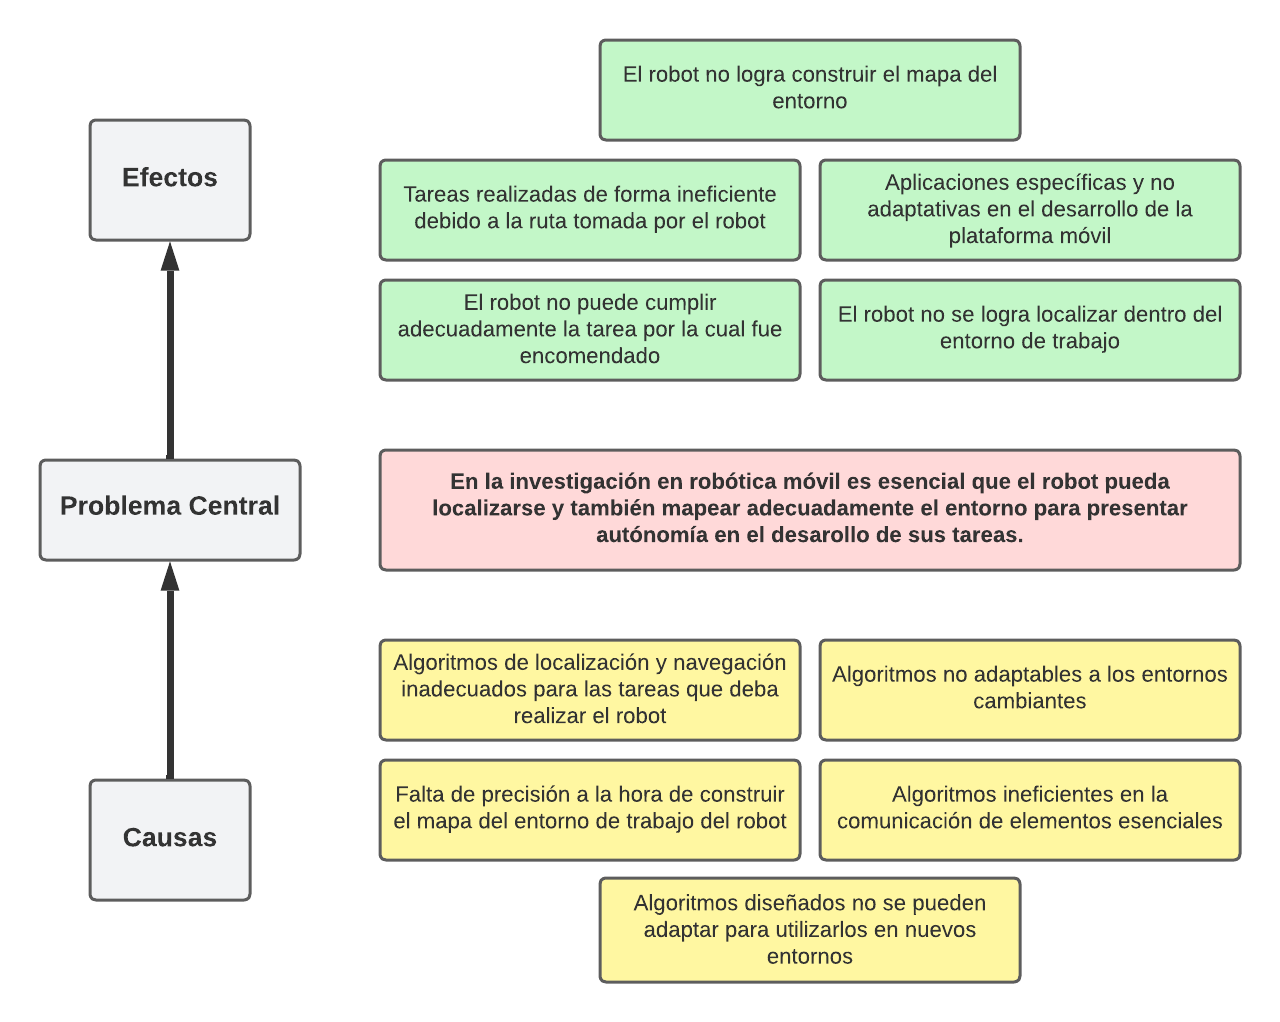
\includegraphics[width=1\textwidth]{figures/01definicion_problema/arbol_del_problema.png}
\caption{\label{fig:arbol_del_problema} Árbol del Problema} Fuente: Fabricación propia
\end{figure}

\subsubsection{SITUACIÓN EN CHILE}

La investigación en robótica en Chile es deficiente y poco desarrollada. Existen menos de una decena de laboratorios de robótica capacitados para la construcción e investigación profesional en el área. Con todo, es importante destacar que existen diversas necesidades que requieren ser satisfechas por la robótica y diversos escenarios o ambientes para poner a prueba los robots. Por otra parte se estima que durante la próxima década cerca del 70\% de la población chilena se encontrará en contacto con algún robot \footnote{A partir del 2018 CONICYT incentiva la investigación en el área de la robótica dando prioridad a los becados interesados en dicha área https://www.conicyt.cl/becasconicyt/2018/03/28/magister-becas-chile-2018-abre-convocatoria-en-areas-de-interes-prioritario/ }. Existen diversos campos de aplicación de esta área, tales como: En la minería analizando y apoyando las labores, en hospitales llevando insumo a las habitaciones, en nuestros hogares cuidándolos mientras no estamos, entre otras más. 

Los campos anteriormente mencionados, tienen como denominador común que el robot para suplir la tarea debe mapear el entorno para luego localizarse y planificar una ruta para realizar la tarea para la cual fue asignado. Bajo esta lógica, es de suma importancia tener algoritmos adaptables a los cambios en el entorno. Por otra parte, se puede observar que la diversidad natural de Chile plantea diversos escenarios que no solo pondrán a prueba los robots a las inclemencias del tiempo, sino también, verificar los algoritmos y el comportamiento de la máquina antes estos escenarios, tal cual como lo ha hecho la \textit{National Aeronautics and Space Administration} con sus \textit{rovers} \cite{wei_autonomous_2015}.

\newpage
\subsection{OBJETIVOS}

El objetivo general de esta memoria consiste en \textit{crear un algoritmo de localización y navegación simultánea utilizando una cámara de profundidad y un lidar para un robot móvil autónomo en ambientes controlados.
}

\subsubsection{OBJETIVOS ESPECÍFICOS}
Para poder cumplir con el objetivo general previamente mencionado, es necesario realizar los siguientes objetivos específicos:
\begin{enumerate}
    \item Analizar los algoritmos de localización y navegación simultánea para adquirir los conocimientos del área a través de una investigación del estado del arte.
    
    \item Diseñar un algoritmo de localización y navegación simultánea tridimensional por medio de la utilización de una cámara de profundidad y un lidar para construir un mapa tridimensional de bajo costo.
    
    \item Evaluar el desempeño del algoritmo propuesto por medio de la implementación física del robot considerando diversos ambientes de pruebas.
\end{enumerate}

\newpage
\subsection{IMPACTO DE SOLUCIONAR EL PROBLEMA}

La investigación en robótica no es algo trivial, pero si es esencial en los tiempos actuales y más aún en los tiempos que se avecinan donde la robótica será un pilar fundamental en la sociedad \cite{rivera_taiba_efectos_2019}. La robótica implica la colaboración de múltiples áreas como lo es la electrónica, la informática y la mecánica, cada una con sus desafíos e implicancia, los cuales deben ser resueltos de manera individual para la creación de un robot. Es por ello, que la metodología de investigación debe ser estructurada y seguir los lineamientos planteados por la comunidad internacional de robótica.

Desde el punto de vista de la informática, uno de los problemas esenciales en la robótica móvil es la navegación, localización y mapeo de un robot en un entorno, siendo aún más complejo dicho desafío en entornos no controlados \cite{fahimi_autonomous_2009}. Ésta es una problemática que requiere ser estudiada y analizada al momento de diseñar un robot móvil autónomo, ya que la movilidad, localización y mapeo son la piedra angular de todo robot autónomo. 

Actualmente, existen una diversidad de algoritmos de localización y navegación simultánea, los cuales tienen requerimientos específicos y están diseñados para suplir necesidades específicas. Estos algoritmos están fuertemente apoyados tanto en los sensores que utilizan los robots, como también en los cambios existentes en el ambiente \cite{omara_indoor_2015}. Por lo que es de suma importancia evaluar el comportamiento de dichos algoritmos y su adaptabilidad a los cambios en el entorno y de esta manera implementar algoritmos de manera eficiente según el ambiente y el requerimiento que se requiere satisfacer.

Es por ello que un análisis exhaustivo a los principales algoritmos de localización y navegación simultánea, evaluar el comportamiento en diversos ambientes a través de distintas métricas estandarizadas por la comunidad mundial y valuar cumplimiento de los requerimientos es de suma importancia en la investigación en robótica \cite{anis_koubaa_robot_2016} y sobretodo, darle solución a las problemáticas esenciales de la técnica (definidas en el estado del arte), ya que de esta manera, además de incentivar la creación de plataformas autónomas móviles para el estudio del área, el análisis permitirá destinar de mejor manera los recursos asociados a la investigación y a su vez, generar una relación entre los requerimientos del sistema y los algoritmos evaluados.

\subsubsection{METODOLOGÍA DE INVESTIGACIÓN}
Tal como se nombró en la sección anterior, la metodología a utilizar debe seguir los lineamientos verificados y comprobados por la comunidad internacional de robótica, ya que de esta manera, se disminuyen los riesgos de quemar componentes, se disminuyen los riesgos de posibles errores estructurales y en casos más graves, poner en riesgo la vida humana. Si bien existen varios puntos de vista sobre la manera más adecuada para la investigación en robótica, la metodología que se utilizará para llevar a cabo la memoria será una de las descritas por \cite{inves_2004}, \textit{`` la metodología del ciclo de vida de Buchanan''}.

El ciclo de vida de Buchanan presenta la estructura que se puede observar en la Figura \ref{fig:Buchanan},
\begin{figure}[h]
    \centering
    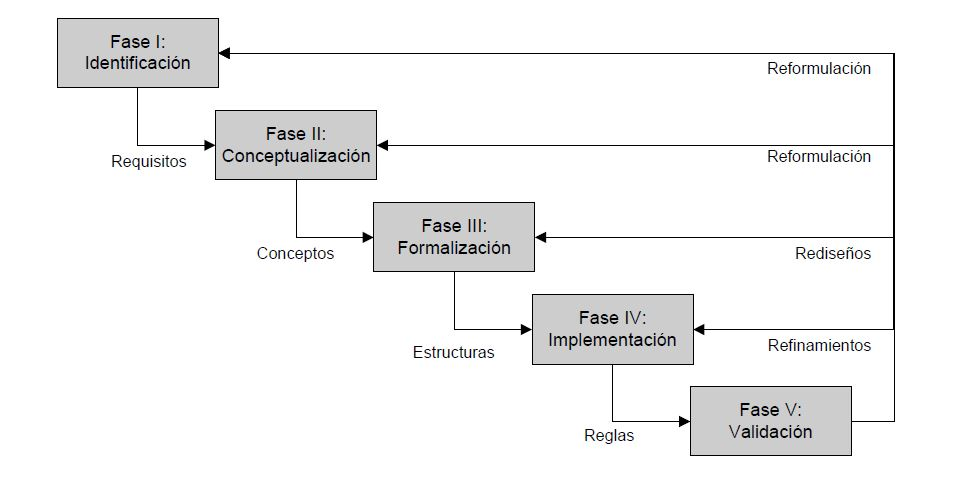
\includegraphics[width=0.8\textwidth]{figures/01definicion_problema/metodologia_Bu.JPG}
    \caption{\label{fig:Buchanan} Metodología del Ciclo de vida de Buchanan} 
    Fuente: \cite{buchanan_2000}
\end{figure}
ya que, producto de los alcances de la memoria y los objetivos planteados es la más adecuada para realizarla. Esta metodología comprende las siguientes fases durante la investigación:
\begin{itemize}
    \item \textbf{Identificación: }Corresponde a la fase inicial en la cual se investiga sobre el estado del arte de la memoria, investigaciones realizadas y sobretodo está centrada en la adquisición de los conocimientos mínimos para la realización de la memoria, en este caso, la investigación del estado del arte de la robótica móvil, investigación sobre el framework ROS e investigar sobre la navegación autónoma. De esta manera se limita los alcances y se determina como se enfrentará al problema de la navegación autónoma.
    \item \textbf{Conceptualización: }Corresponde a la continuación de la fase anteriormente descrita en donde se definen los problemas en concretos que se deben resolver, de esta manera, se definen los conceptos más relevantes que deben ser tratados en la memoria, como por ejemplo, los conceptos de localización y navegación en la robótica móvil autónoma. También se deben reconocer las estrategias que se utilizarán para dar solución al problema.
    \item \textbf{Formalización: }Una vez que se construye el marco teórico, en la fase de la formalización, se dará pie a organizar la información recaba y los conocimientos adquiridos para dar pie a la realización del primer prototipo (diseño) que da solución al problema o los problemas identificados en las fases anteriores.
    \item \textbf{Implementación: }Corresponde a la fase dónde se implementa propiamente tal el prototipo diseñado en la fase anterior, es una fase iterativa dónde se ajustan los parámetros, se implementan los diversos algoritmos investigados y se realizan las diversas estrategias planteadas anteriormente. 
    \item \textbf{Validación: }La última fase corresponde a la fase de validación en dónde, el prototipo se validará frente a diversas situaciones y ambientes, de esta manera se corroborará que la investigación fue la adecuada para resolver los objetivos descritos.
\end{itemize}



